\documentclass[a4paper, 10pt]{scrreprt}


\usepackage[ngerman]{babel}
\usepackage[utf8]{inputenc}


\usepackage{hyperref}

\usepackage{graphicx}



\newcommand{\scenario}[5]{
\begin{description}
\item [\uppercase{Initiale Situation}:]#1
  \item [\uppercase{Normal}:] \textit{#2}
  \item [\uppercase{Was schief gehen kann}:] \textit{#3}
  \item [\uppercase{Andere Aktivitäten}:] #4
  \item [\uppercase{Zustand des Systems bei Erfolg}:] #5
\end{description}
}



\newcounter{UReqCounter}
\newcommand{\ureq}[2]{%
  \vspace{0.5em}%
  \stepcounter{UReqCounter}\noindent%
  \textbf{U-REQ \arabic{UReqCounter}:} #1 \textit{Priority: #2}
}

\newcounter{FReqCounter}

\newcommand{\freq}[3]{%
  \vspace{0.5em}%
  \stepcounter{FReqCounter}\noindent%
  \textbf{F-REQ \arabic{FReqCounter}:} #1
  \textit{U-REQ #2}
  \textit{Priority: #3}
}

\newcounter{NFReqCounter}

\newcommand{\nfreq}[2]{%
  \vspace{0.5em}%
  \stepcounter{NFReqCounter}\noindent%
  \textbf{NF-REQ \arabic{NFReqCounter}:} #1 \textit{Priority: #2}
}





\setcounter{secnumdepth}{5}

\setcounter{tocdepth}{10}



%Glossaries

\usepackage{glossaries}
\usepackage{glossaries-extra}

\makenoidxglossaries

%TODO Glossar - beständig ergänzen

%FIXME

\newcommand{\glx}[1]{#1 \gls{#1}}

\newglossaryentry{Admin}{name={Admin},description={
Der Admin (-istrator) in diesem Dokument ist der Leiter und Verwalter von Experimenten.}}

\newglossaryentry{Experiment}{name={Experiment},description={
Das Experiment ist der Vorgang in dem Clients eine Frage beantworten, darüber diskutieren, evtl. ihre Antworten ändern und alles vom Admin ausgewertet wird.} }

\newglossaryentry{Frage}{name={Frage},description={
Die Frage ist die Grundlage eines jeden Experiments.}}
                                                                                   
\newglossaryentry{Client}{name={Client},description={
Clients sind die Personen, die als ProbandInnen an Experimenten teilnehmen. Die Clients entsprechen den Benutzern.
Das sind die Personen, die sich registrieren, Fragen beantworten und diskutieren.}}

\newglossaryentry{Gruppe}{name={Gruppe},description={
Die Gruppe ist eine Einteilung von Clients nach verschiedenen Charakteristika.}}

\newglossaryentry{Charakteristik}{name={Charakteristik},description={
Charakteristika entsprechen den vom Client angegebenen Profilinformationen}}

\newglossaryentry{Diskussion}{name={Diskussion},description={
Diskussionen sind der Austausch zwischen Clients, anhand derer eine eventuelle Beeinflussung gemessen werden kann.}}

\newglossaryentry{Aktivitaetsscore}{name={Aktivitätsscore},description={
Der Aktivitätsscore soll die Maßeinheit sein, in der eine eventuelle Beeinflussung von Clients gemessen wird.}}

\newglossaryentry{Chat}{name={Chat},description={
Der Chat ist ein sogenanntes Instant-Messaging-Programm wie z.B. WhatsApp.
Über den Chat werden die Diskussionen geführt.}}

\newglossaryentry{Chatverbindung}{name={Chatverbindung},description={
Die Chatverbindung ist die Kommunikationserlaubnis zwischen zwei Clients.}}

\newglossaryentry{App}{name={App},description={Für Clients bereit gestellte Andoid App, die über den Google Play Store/von unserem Laptop aus, weil wir keinen PLay Store Account haben installiert wird.}}

\newglossaryentry{Datenbank}{name={Datenbank},description={Der Server speichert die Daten anonym und sicher}}

% Document information

\title{Lastenheft}

% \author{Jaqueline K. \and Nicole W. \and Rebecca K. \and Lucas B.}
\author{Gruppe H}

\date{\today}


\begin{document}
\maketitle


\tableofcontents


\begin{abstract}
 
Es soll eine datenbankbasierte Android-App entwickelt werden, 
mit deren Hilfe man analysiert, inwiefern Netzwerk-Topologien individuelle Entscheidungen von sog. Clients beeinflussen. 
Ein Client ist ein Teilnehmer bzw. Benutzer der App, der bestimmte Fragen beantwortet und Diskussionen mit anderen Clients führt. 
Diskussionen zwischen Clients sind Chats, über die z.B. auch Bilder oder anderes Informationsmaterial ausgetauscht werden kann. 
Die andere Gruppe von Benutzern sind die Personen, die diese Experimente durchführen (Admins). 
Diese sollen dazu in der Lage sein, die zu beantwortenden Fragen zu definieren und diese für bestimmte Clientgruppen freizugeben. 
Die Freigabe soll dabei für Clients mit bestimmten Merkmalen erfolgen können (z.B. für alle Clients mit Kindern zwischen 20 und 30 Jahren). 
Zur anschließenden Analyse soll ein filterbarer Datenexport bereitgestellt werden.

\end{abstract}


%\chapter{Introduction}

%FIXME Entweder Intro oder Abstract




\chapter{Introduction}

\section{(Initial) Problem Statement for the Mobile Decision Lab}
The purpose of the system is to have a mobile lab for experiments concerning groups decisions based on different network topologies. The outcome of experiments shall help understand how network structures impact group decisions. The networks are anonymous connections between participants with the possibility to exchange messages between connected participants.

Networks can be constructed, for instance, scale-free or not, or with certain dimensionalities (everyone has exactly one neighbor, exactly two neighbors, etc.) and in a way that they additionally fulfill certain constraints (e.g., a connection between two participants {\em can only exist} if they share some properties, e.g., they are about the same age or have about the same expertise about the subject matter, or such a connection {\em cannot exist} if certain properties hold, e.g., neighbors have to be in different age groups or they are not allowed to have the same level of expertise).

The message format can be plain text or more structured, like an integer, or an enumeration type (like ``up'' or ``down'' or a chess move or a (legal) sentence like ``guilty'' or ```not guilty''').

There are two types of users of the systems: experimenters (admins) or participants (test persons, subjects). Experimenters define the experiments along with all parameters and constraints. Participants can register and decide whether they want to participate in a given experiment. Before the start of the experiment, participants have to answer a few questions related to the task they should solve. (If no such information is requested by the experimenter in the definition of the experiment, this step can be omitted. Answers to these questions are treated confidentially, as all the other information that is entered by participants of the experiments.) Once the experiment has started, they are provided with a task description, which is the problem to be solved and for which a decision has to be reached towards the end of the ``game'' (i.e., has to be entered by each participant individually), and some supporting information (for instance, some paragraphs of law text for legal problems, or a hint on which supporting information they are allowed to use, e.g., some news website or wikipedia articles).

During one round of deliberation, participants can exchange messages with their (anonymous) neighbors about the problem to be solved, according to their own pace, until the predefined time of the experiment is up or the experimenter decides to close the experiments manually. 

When the time of deliberation has ended, each user is asked to decide about the question he or she was asked to answer in the beginning. The answer will be of a predefined format (not free text).

The nature of the experiment should be such that a ``true'' outcome is known already, but hard or impossible to access by participants (like a known sentence for a known case in the legal setting), or will be known shortly in the future (like the outcome of a football game or a chess move by a professional chess player in a certain game or the loss or gain of a stock on the stock market on the next day).

At the end of the experiment, the outcome of the decision (for instance, the fraction of participants choosing ``guilty'' or ``not guilty'' or the fraction predicting the win or loss of a forthcoming football game) can be communicated to the participants, if the experimenter has chosen this option up-front in the definition of the experiment.

All the results, the individual decisions and the group decisions are stored in a database in anonymized form for future analysis.

An experiment can be defined in a way that it is repeated with the same group of people and the same or, alternatively, a different network topology for a specified number of times. These are parameters specified by the experimenter up-front, before the experiment has started.

The outcome that was known already, but hard to access, or that is only known shortly after the experiment has ended, can also be communicated to the participants, if the experimenter wishes to do so.

\subsection{Experimenter Perspective}
The experimenter (also known as the admin) can define an experiment (for details see above) and access the results. When the experiment is defined, the questions to be answered by the participants can be specified, the task description, the supporting information, parameters specifying the network type, parameters regarding the repetition of experiments, and the duration of the experiment (predefined or stopped manually). 

In the first step, the questions to be asked are defined (e.g., ``Are you older than 40?''). The answers serve as background information on the participants, but can also be used as constraints in the automatic and randomized construction of the network. For example, everyone could be connected only to people who are older or younger. Once the network is constructed, a decision problem is sent to the users (along with some material that may help in the decision). The admin can set a time frame for the deliberation or stop the experiment manually at any time. After the time is up or the experiment is stopped manually, and the decisions are entered by all participants, the experimenter has access to the outcomes in anonymized form.

\subsection{Participant Perspective}
The participant can sign up for the mobile decision lab in an android app. He/she may select an experiment to participate in. The participant then has to answer some preliminary questions. After that the participant is presented with a decision problem along with additional material. The participant studies the material and exchanges information and opinions with other participants he/she is connected to in the participant network. Information exchange only happens between two participants at a time. The message format may be different from experiment to experiment. In the simplest case, it is just plain text. After some time of deliberation (discussion of neighboring participants by exchanging messages), the participant is asked to make a final decision. After the decision is made, the participant may get some feedback on her answer depending on the experiment setup (the experiment could also be set up in a way that the participant does not receive feedback). Depending on the user's participation in the experiment, he/she may receive a number of points after each question. The participant can compare his/her performance with other participants on a global leader board. This scoring system is optional and may be chosen by the experimenter in the specification of the experiment.



%\section{Glossar}

\printnoidxglossary[sort=word]

%Ungenutzte Einträge funktioniert leider noch nicht.

%\printunsrtglossaries

\part{User Requirements (aus der Musterlösung)}

\chapter{System Administrator and Experimenter}
The experiments are set up and managed by the experimenters. 
However, to grant user rights and deal with unwanted behavior by experimenters, the role of the system administrator is needed.

\section{System Administrator}
\ureq{The system administrator should be able to give rights to users to make them experimenter. (Each user should be manually confirmed as an experimenter. Experimenter privilege is restricted to selected individuals.)}{B}

\ureq{The system administrator should be able to take away the experimenter status either permanently or for a specified time frame (An experimenter may lose his/her privilege by setting up too many experiments or otherwise abusing the system).}{C}

\section{Sign-up process}
Since the experimenters have more rights than other participants, it is recommended to ask the experimenters for additional information during the sign-up process.

\ureq{The experimenters shall be able to sign up as normal users that additionally select an option for wanting to become an experimenter.}{B}

\ureq{The experimenters should be asked for additional information during sign-up: their real name, a description of the intended usage of the system, their field of study, and their associated university. (While this information can be kept optional, it may help to evaluate system usage at a later point.)}{B}

\ureq{The experimenters shall be able to sign in with a username and password.}{A}

\ureq{The experimenters shall be able to request a new password.}{B}

\section{Experiment setup}
Every experiment needs careful setup. Since the aim of the experiment is to create useful data, which can be further processed by applying scientific methods, all settings and setting changes, if applicable, have to be carefully monitored so they may be retraced at a later time.

\subsection{General}

\ureq{The experimenters shall be able to set up a \textit{new experiment}.}{A}

\ureq{The experimenters shall be able to define the \textit{task description}. (The task description provides information on the experiment without giving away the central question.)}{A}

\ureq{The experimenters shall be able to set up the used \textit{language} for the given experiment. (English should be the default language, but other languages should be possible as well.)}{A}

\ureq{The experimenters shall be able to define one or more \textit{preliminary questions} for the experiment. (It is also possible to have no preliminary questions.)}{A}

\ureq{The experimenters shall be able to define the \textit{central question} for the experiment along with a list of possible answers or an intended answer format (e.g. an integer to specify the number of years a defendant should be sent to prison).}{A}

\ureq{The experimenters shall be able to enter the \textit{correct answer} for the central question. (This may happen in the beginning, during the course of, or after the experiment has finished.))}{}

\ureq{The experimenters shall be able to provide \textit{additional information} for the given experiment by uploading a description and the content itself. (E.g. for a legal decision the text of certain laws or a surveillance video or a list of previous offenses of the defendant would be possible additional information. It may be in the form of links or pdfs, but also images, videos or other file formats should be possible.)}{B}

\ureq{The experimenters shall be able to define the \textit{number of experiments} to be performed in a sequence. (It may be interesting to study the behavior of the same group of people during the course of a series of experiments.)}{A}

\ureq{The experimenters shall be able to repeat the same experiment with different parameters. (This means the experiment could be repeated with the same question and different network topologies or different questions and the same or a different network topology.)}{A}

\subsection{Social network}

\ureq{The experimenters shall be able to define parameters specifying the \textit{network type}. (E.g. the network should be scale-free or not or have a specified number of connections between any two users.)}{A}

\ureq{The experimenter shall be able to define the \textit{message format} for the user messages. (Messages could be plain text, but other formats such as numbers or more structured formats must also be possible.)}{A}

\subsection{Start and End}

\ureq{The experimenters shall be able to define start \textit{time and duration} of the experiment.}{A}

\ureq{The experimenters shall be able to set a time frame for the \textit{deliberation}. (The central question is available once the deliberation begins. The deliberation may only begin after the experiment has enough participants, the network is defined, and the central question along with the additional material is available.)}{A}

\ureq{The experimenters shall be able to \textit{stop} the experiment manually at any time with or without requiring to answer the central question. (E.g. if a football game is canceled, and the central question is on the results of the game, it does not make sense to ask users to answer the question anymore.)}{A}

\subsection{Statistics}

\ureq{The experimenters shall be able to decide whether the experiment will contribute points to a \textit{global leader board}. (Some experiments may require that users are not influenced by a desire to score points on the leader board.)}{B}

\ureq{The experimenters shall be able to define whether the correct answer and \textit{answering statistics} are presented to the user at the end of the experiment. (In a series of experiments it might make sense to only present results after the series has finished.)}{A}




\section{Experiment - Results}
The results of the experiments have to be accessible to the experimenters without violating privacy rights.

\ureq{The experimenters shall be able to access the outcomes of the experiment in anonymized form.}{A}

\ureq{The experimenters shall be able to download the outcomes of the experiment.}{C}

\ureq{The experimenters shall be able to save the outcomes of the experiment in anonymized form.}{A}

\section{Troubleshooting}
A system can break down due to all kinds of errors and unexpected situations. This is where the system administrators need to step in. To give experimenters the means to inform the system administrators, the following rights are needed:

\ureq{The experimenters shall be able to contact the system administrators.}{A}

\chapter{Participants/User}

This software is supposed to create an appealing environment for users and guarantee simple and intuitive usage to ensure the success of the experiments.

\section{Sign-up and Sign-in}
To ensure a quick start for the user, we want to provide the possibility of logging in with an existing accepted account. Since every user needs to have a clear identity, we need to ensure that every user is registered in the system and is able to keep his identity safe.

\ureq{The user shall be able to sign-up using his email, thus creating a user name and password}{A}

\ureq{Each user shall only be able to sign up once. (This ensures the credibility of the experiment outcome}{A}

\ureq{The user shall be prompted to accept the privacy policies.}{A}

\ureq{The user shall be able to request a new password.}{B}

\ureq{The user shall be able to start the tutorial. (A tutorial facilitates quick adoption of the main principles of the app without requiring to participate in a real experiment. Thus it prevents users from enrolling in experiments without the intention to complete them.)}{D}

\ureq{The user shall be able to quit the tutorial.}{D}

\ureq{The user shall be able to use an existing verified and accepted account as login data. (e.g. a Facebook account.)}{D}

\section{Experiment Management}

\ureq{The user shall be able to read the descriptions of all available experiments.}{A}

\ureq{The user shall be able to choose from a list of available experiments.}{A}

\ureq{The user shall be able to access a list of experiments that he/she currently participates in.}{A}

\ureq{The user shall be able to view the status of each experiment that he/she currently participates in. (E.g. to see if the deliberation period has already started or ended.)}{B}

\section{Questions}
Core element of the experiment is the answering of questions by users.

\ureq{The user shall be able to answer the preliminary questions after choosing to participate in an experiment.}{A}

\ureq{The user shall be able to see the intended time of the deliberation period.}{A}

\ureq{The central question must be readable by the user once the deliberation period has started.}{A}

\ureq{It must be possible for the user to answer the central question once the deliberation period is over.}{A}

\ureq{After the end of the deliberation period, the user has to be able to answer the central question until the end of the given deadline.}{A}

\ureq{Once the deliberation period has ended the user shall be able to see the remaining time for answering the question. (E.g. after a deliberation period of one week, a countdown starts and the question has to be answered within one day.)}{B}

\ureq{The user shall be able to access or download additional material that may help in answering the central question.}{A}

\ureq{The user shall be able to see the correct answer after the end of the experiment if the experimenter has allowed it in the experiment setup.}{B}

\section{Options}
In addition to participating in the experiments, each user has the opportunity to control certain aspects of the app using predefined options.

\ureq{The user shall be able to access the settings menu of the app.}{B}

\ureq{The user shall be able to modify the appearance of the app.}{D}

\ureq{The user shall be able to contact the system administrator.}{C}

\ureq{The user shall be able to specify his/her spoken languages.}{A}

\section{Message System}
One part of the general setup of each experiment is the opportunity to exchange messages during the deliberation period of the experiment.

\ureq{The user shall be able to see the usernames of people he/she is connected to in the social network.}{A}

\ureq{The user shall be able to send messages to other users in the network if he/she is connected to them in the social network during the deliberation period.}{A}

\ureq{The user shall be able to contact an experimenter (This may be necessary to report abuse, spam etc.).}{B}

\ureq{The user shall be able to mute a contact. (This is necessary to prevent trolling.)}{B}

\ureq{A profanity filter should verify messages (This only applies if messages contain plain text).}{B}

\ureq{The user shall have the option to send a message to multiple users at once. (This facilitates communication especially when the network is densely connected.)}{B}

\section{Leaderboard}
Another incentive to use the app is the leader board. Competition ensures that users keep answering the questions and engage in discussions.\\

\ureq{The user shall be able to see the global ranking.}{C}

\ureq{The user shall be able to see his/her own rank.}{C}

\chapter{System specification}
Independent of its users, the system should conform to the following requirements.

\ureq{The system shall be accessible through a web browser.}{A}

\ureq{The system shall be accessed through a mobile phone app.}{A}

\ureq{The system shall comply with ethical guidelines for experiments in the social sciences.}{A}

\ureq{All data shall be stored according to the highest security standards.}{A}



%bis hier entfernen für Endversion

\part{System Requirements}




\chapter{Non-Functional Requirements}


\section{Product Requirements}

\begin{figure}
 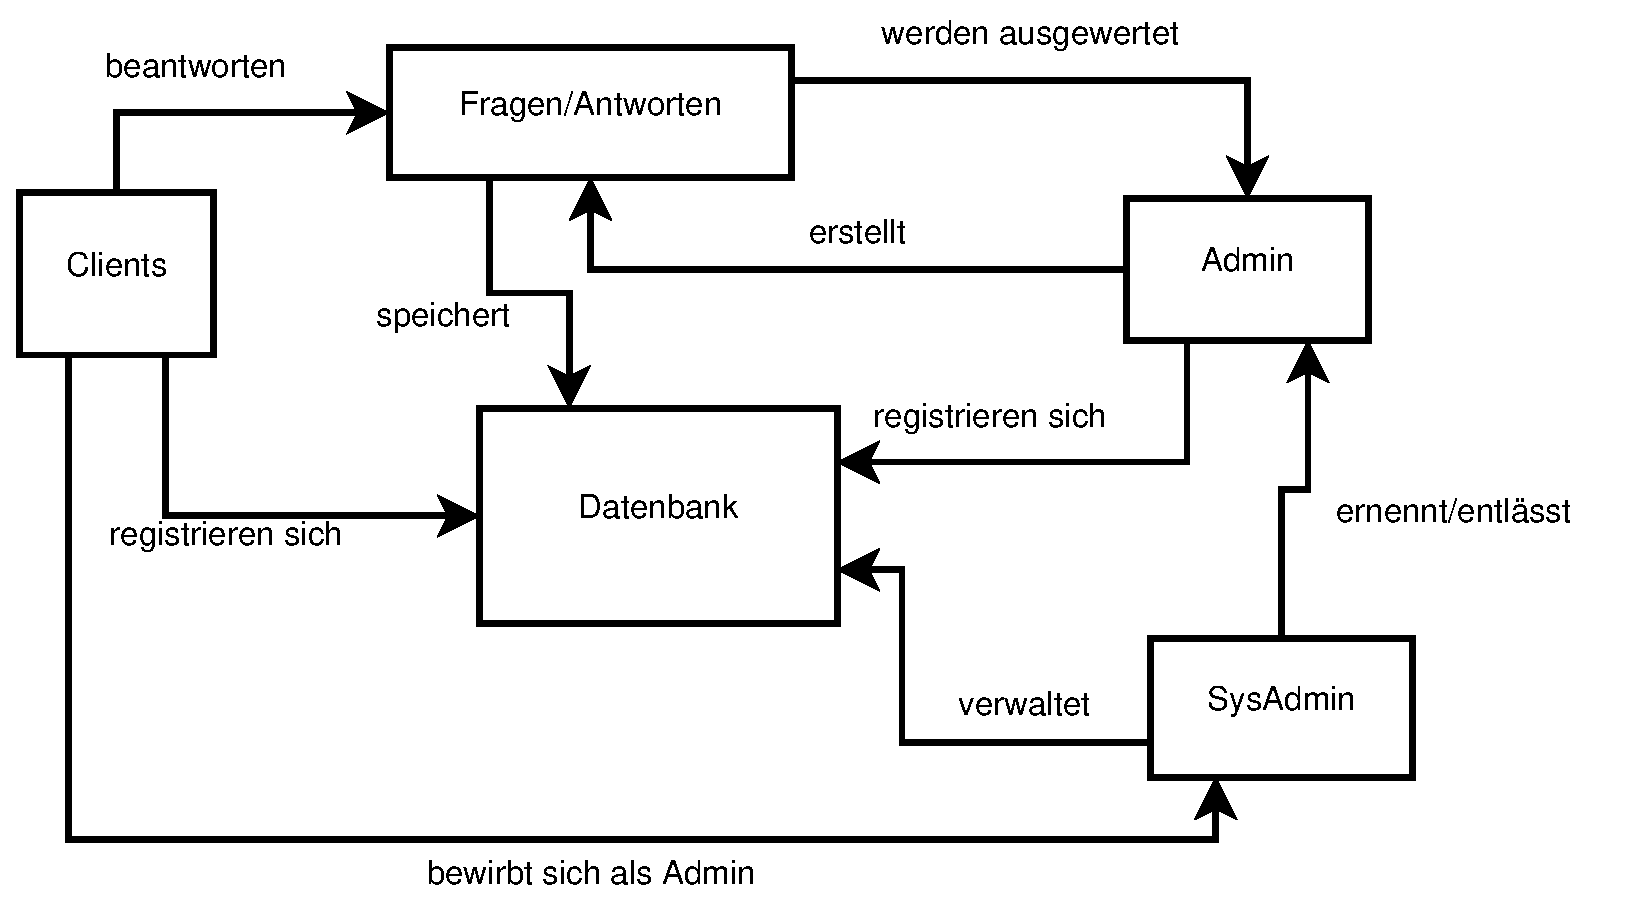
\includegraphics[width=\textwidth]{./pics/Diagramm1e.eps}
 % Diagramm1e.eps: 0x0 pixel, 300dpi, 0.00x0.00 cm, bb=0 0 765 425
 \caption{Übersicht: Zusammenarbeit der Komponenten}
 \label{abb:1}
\end{figure}


\subsection{Dependabiblity Requirements}
\nfreq{Ein wartungsbedingter Ausfall sollte nicht länger als 10 Minuten andauern.}{A}

\subsection{Security Requirements}
\nfreq{Das System sollte gegen herkömmliche Hackerangriffe resistent sein.}{A}

\nfreq{Das System sollte mit Schutzmechanismen gegen Bots und vandalisierende Benutzer ausgestattet sein.}{A}

\nfreq{Benutzerkritische Daten (wie z.B. Passwort) sollten mit einer zeitgemäßen Verschlüsselungsmethode verschlüsselt sein.}{A}


\section{Usability Requirements}
\nfreq{Die Weboberfläche des Systems soll mit allen gängigen Browsern darstellbar sein.}{A}

\nfreq{Die App soll mit allen Android-Geräten fehlerlos funktionieren.}{A}

\nfreq{Alle potentiellen Nutzer sollen das System innerhalb von 10 Minuten (mit Tutorial) verstehen können.}{A}

\nfreq{Alle potentiellen Admins sollen das System innerhalb von 30 Minuten verstehen können.}{A}


\section{Efficiency Requirements}
\nfreq{Systemseitige Prozessse (wie z.B. die Erstellung oder Beantwortung einer Frage) soll nicht länger als 1 Sekunde dauern (falls eine stabile Internetverbindung besteht).}{A}

\nfreq{Aufwändige Operationen (wie z.B. der Export von 5 MB Daten) sollen in weniger als 5 Sekunden abgeschlossen sein.}{A}


\section{Performance Requirements}
\nfreq{Es sollen mindestens 5000 User gleichzeitig am System arbeiten, ohne dass es zu verzögerten Wartezeiten kommt (5 Sekunden länger als normal).}{A}

\nfreq{Die Datenbank soll ohne Beeinträchtigunngen der Performance mindestens 100GB Daten enthalten können.}{A}



\chapter{Funktionale Anforderungen}

\section{Technische Anforderungen}

\freq{Wir verwenden eine Postgre-SQL Datenbank.}{1}{A}

\freq{Das System soll eine Weboberfläche zur Verfügung stellen.}{58}{A}

\freq{Das System soll über eine mobile App benutzbar sein.}{59}{A}

\freq{Die Datenbank erfüllt zeitgemäße Sicherheitsstandards.}{61}{A}

\freq{In der Datenbank existiert eine erweiterbare Tabelle mit Sprachen.}{9}{A}

\freq{Die Datenbank ist in der Lage einen Export bestimmter Daten zur Verfügung zu stellen. \gls{Admin}s können diese herunterladen.}{24}{C}

\freq{Siehe F-REQ 6.}{25}{A}

\freq{Die Datenbank ist in der Lage für jeden Admin einen Wiederherstellungs-Code zu generieren, über den er ein neues Passwort festlegen kann.}{6}{A}

\freq{Die Datenbank ist in der Lage für jeden Client einen Wiederherstellungs-Code zu generieren, über den er ein neues Passwort festlegen kann.}{30}{A}

\freq{Es gibt eine API-Schnittstelle zu anderen Datenbanken (z.B. Facebook), über die Benutzer-Account exportiert bzw. importiert werden können.}{33}{D}




\section{Sonstige technische Anforderungen}
\freq{Das System stellt ein (Video-)Tutorial für neue Benutzer bereit.}{31}{D}


\freq{Benutzer können das Tutorial überspringen bzw. beenden.}{32}{D}


\freq{Das System soll über verschiedene Einstellungen verfügen.}{46}{B}


\freq{Diese Einstellungen sollen individuell von Benutzern konfiguriert werden können.}{47}{D}


\freq{In den individuellen Einstellungen können Clients ihre bevorzugte Sprache konfigurieren.}{49}{A}






\section{Benutzer (betrifft alle Rollen)}
\freq{Benutzer können sich (mit E-Mail-Adresse, Benutzername und Passwort) am System registrieren und ihren Account verwalten. Dazu gibt es eine Benutzer-Tabelle in der Datenbank.}{27}{A}


\freq{Dadurch, dass Admins in der gleichen Tabelle stehen, in der auch alle Clients sind, sind diese auch automatisch Clients.}{3}{A}


\freq{Es gibt in der Benutzer-Tabelle einen Unique-Key mit Benutzername bzw. E-Mail Adresse.}{28}{A}


\freq{Bei der Registrierung wird ein Benutzer aufgefordert, die Nutzungsbedingungen zu akzeptieren.}{29}{A}




\section{SysAdmins}
\freq{SysAdmins haben Zugriff auf die gesamte Datenbank und können (markierte) Clients zu Admins befördern. Sie können den Admin-Status auch wieder entfernen.}{2}{A}


\freq{Admins sind über das System in der Lage, SysAdmins zu kontaktieren (z.B. per Kontaktformular).}{26}{A}


\freq{Clients sind über das System in der Lage, SysAdmins zu kontaktieren (z.B. per Kontaktformular).}{48}{C}




\section{Admins}
\freq{Die Admins stehen ebenfalls in der gleichen Benutzer-Tabelle und sind über ein Boolean-Feld gekennzeichnet.}{1}{A}


\freq{Für Admins können in der Datenbank zusätzliche Informationen gespeichert werden (Name, Grund für die Nutzung des Systems, Universität, Studienfach).}{4}{A}


\freq{Der Admin wählt experimentbezogen eine Sprache aus. Diese wird in der Experiment-Tabelle hinterlegt. (Default: Englisch.)}{9}{A}


\freq{Clients sind über das System in der Lage, Admins zu kontaktieren (z.B. per Kontaktformular).}{52}{B}


\section{Clients}
\freq{In der Benutzer-Tabelle gibt es ein Boolean-Feld über das ein Client sich für den Admin-Status bewerben kann.}{1}{B}


\freq{Für jeden Client wird in der Datenbank der Benutzername und ein Passwort gespeichert.}{5}{A}


\freq{In der Benutzer-Tabelle existiert ein Feld für den \gls{Aktivitaetsscore}.}{21}{B}

\freq{In der Compound-Tabelle existiert ein Boolean-Feld, über das die \gls{Chatverbindung} stummgeschaltet werden kann.}{53}{B}

\freq{Das System stellt eine globale Rangliste aller Clients mit deren Aktivitätsscore zu Verfügung (in absteigendender Reihenfolge).}{56}{C}


\freq{Das System zeigt Clients ihre Position in der globalen Rangliste an.}{57}{C}




\section{Experiment-Erstellung}
\freq{Die Datenbank speichert die durch Admins erstellte Experimente in einer Tabelle.}{7}{A}


\freq{In der Experiment-Tabelle gibt es ein Feld zur Eingabe der Experiment-Beschreibung.}{8}{B}


\freq{Eine zu den Experimenten verlinkte Tabelle speichert "preliminary questions".}{10}{A}


\freq{Das System akzeptiert Antworten auf "preliminary questions" nur von am Experiment teilnehmenden Benutzern.}{38}{A}


\freq{In der Experiment-Tabelle kann in einem Feld vom Admin die eigentliche Frage hinterlegt werden.}{11}{A}


\freq{In der Experiment-Tabelle kann in einem Feld vom Admin der Antworttyp eingetragen werden (Multiple-Choice, Datum, Zahl, Boolean).}{11}{A}


\freq{Admins können zu Ihren Fragen Dokumente in bestimmten Formaten (PDF, JPG, PNG, ...) hochladen.}{13}{A}


\freq{In der Experiment-Tabelle kann in einem Feld (eins je Antworttyp) vom Admin die korrekte angegeben werden.}{12}{A}


\freq{In der Datenbank gibt es eine Sequenz-Tabelle, in der eine Abfolge von Experimenten gespeichert werden kann.}{14}{C}


\freq{In der Datenbank gespeicherte Fragen können von Admins kopiert werden, wobei Parameter geändert werden können (z.B. preliminary questions, Dokumente, Beschreibung, ...).}{15}{A}


\freq{In der Experiment-Tabelle existiert ein Boolean-Feld, das angibt, ob diese Frage den Aktivitätsscore beeinflusst (vom Admin festgelegt).}{21}{B}




\section{Stati von Experimenten}
\freq{In der Experiment-Tabelle gibt es Felder den Start- und Endzeitpunkt (vom Admin festgelegt).}{18}{A}


\freq{In der Experiment-Tabelle gibt es ein Feld für die Bedenkzeit (vom Admin festgelegt).}{19}{A}


\freq{Das System zeigt jedem teilnehmenden Client den Wert der verbleibenden Bedenkzeit an.}{39}{A}

\freq{Das System zeigt jedem teilnehmenden Client nach der Bedenkzeit die verbleibende Antwortzeit bis zum Endzeitpunkt an.}{43}{B}

\freq{In der Experiment-Tabelle gibt es ein Boolean-Feld für die Markierung von inaktiven Experimenten (vom Admin festgelegt).}{20}{A}

\freq{Das System zeigt den teilnehmenden Clients die eigentliche Frage nur während der Bedenkzeit an.}{40}{A}

\freq{Das System ermöglicht teilnehmenden Clients nach der Bedenkzeit die Eingabe der Antworten.}{41}{A}

\freq{Das System sperrt die Antworteingabe nach dem Endzeitpunkt des Experiments.}{42}{A}


\section{Experiment-Übersicht}
\freq{Es gibt für Clients eine filterbare Übersicht aller Experimente mit deren Beschreibungen.}{34}{A}

\freq{Das System stellt Clients eine Übersicht der Experimente bereit, an denen sie teilnehmen können.}{35}{A}

\freq{Das System stellt Clients eine Übersicht der Experimente bereit, an denen sie aktuell teilnehmen.}{36}{A}

\freq{In der Experiment-Übersicht für Clients soll der Start- und Endzeitpunkt bzw. Status (aktiv / inaktiv).}{37}{B}


\freq{Teilnehmende Clients sollen in der Lage sein, die hochgeladenen Dokumente herunterzuladen.}{44}{A}


\section{Experiment-Ergebnis}
\freq{Die Datenbank speichert die Antworten in einer Antwort-Tabelle, in der die User-IDs der beantwortenden Personen verschlüsselt sind.}{23}{A}

\freq{Teilnehmende Clients sollen (falls vom Admin so definiert) in der Lage sein, nach dem Endzeitpunkt die korrekte Antwort einer Frage zu sehen.}{45}{B}

\freq{In der Experiment-Tabelle muss vom Admin festgelegt werden können, ob das Ergebnis nur ihm, öffentlich, oder nur bestimmten Usern zur Verfügung steht.}{22}{A}




\section{Netzwerk}
\freq{Es gibt in der Datenbank eine Compound-Tabelle, die die Netzwerk-Topologie speichert (\gls{Chatverbindung}en).}{16}{A}

\freq{In der Compound-Tabelle gibt es mehrere Boolean-Felder für das Nachrichtenformat, das vom Admin festgelegt wird.}{17}{A}

\freq{Wenn eine Chatverbindung im System besteht, können die beteiligten Clients gegenseitig ihre Benutzernamen sehen.}{50}{A}

\freq{Wenn eine Chatverbindung im System besteht, können beteiligte Clients während der Bedenkzeit Nachrichten austauschen.}{51}{A}

\freq{Das System stellt eine geeignete Filterfunktion für unangemessene Ausdrücken in Chats zur Verfügung.}{54}{B}

\freq{Das System ermöglicht die gleichzeitige Auslieferung einer Nachricht an mehrere Clients in Form einer "Rundnachricht".}{55}{B}


\section{Ethische Leitlinien}

\freq{Das System soll ethischen Leitlinien unterliegen.}{60}{A}




\part{Szenarios}

\chapter{Szenario für die Erstellung eines Experiments}

\scenario{Ein \gls{Admin} möchte ein \gls{Experiment} erstellen: Wie lange muss ein verurteilter Täter in Haft? Dazu lädt er eine PDF-Datei mit Informationen zum Tathergang und dem Urteil hoch und ordnet eine \gls{Gruppe} dieser Frage zu.}
{\begin{itemize} 
  \item Der Admin benutzt das Experiment-Erstellungs-Interface und gibt die Frage, die Antwortmöglichkeit als Kommazahl und eine Fragebeschreibung (z.B. Bitte zugeordnetes PDF beachten. Kommazahlen als Antwort sind erlaubt.) ein.
  \item Der Admin gibt außerdem einen Zeitraum für das Experiment, sowie die Dauer für Clients, eine Antwort abgeben zu können, an.
  \item Der Admin lädt das Info-PDF hoch.
  \item Der Admin sucht eine Gruppe aus und ordnet diese zu. (z.B. Jura-Studenten)
  \end{itemize}}
{\begin{itemize}
    \item Die Eingaben (Fragetext und Fragebeschreibung) könnten zu lang sein (Speicher für das Feld in der Datenbank reicht nicht aus).
    \item Das PDF könnte zu groß oder im falschen Format sein.
    \end{itemize}}
{Zu viele andere Zugriffe könnten den Server überlasten und zu einem Ausfall führen.}
{User ist eingeloggt. Die Frage ist erstellt und wird mit PDF und allen weiteren vom Admin eingegebenen Infos den ausgewählten Clients zur Teilnahme bereitgestellt.}

\chapter{Szenario für die Registrierung als Client}

\scenario{Eine Person möchte sich über die \gls{App} als \gls{Client} registrieren.}
{\begin{itemize} 
  \item Die Person installiert die App über den Google Play Store.
  \item Sie startet die App, die sich mit dem Server verbindet und einen Registrierungsbildschirm anzeigt.
  \item Sie wird aufgefordert die für die Registrierung erforderlichen Daten einzugeben. Sie gibt diese ein und bestätigt die Übermittlung an den Server.
  \item Der Server speichert die Eingaben in der \gls{Datenbank} und meldet die erfolgreiche Registrierung zurück.
  \end{itemize}}
{\begin{itemize}
    \item Die App ist für das verwendete OS nicht verfügbar.
    \item Die App ist zwar verfügbar, läuft aber auf dem verwendeten System nicht.
    \item Die App läuft unbrauchbar langsam.
    \item Es ist keine Verbindung zum Server möglich.
    \item Der Server ist überlastet.
    \item Ein frei wählbarer Bezeichner, der als Schlüssel für die Datenbank verwendet wird, ist schon belegt.
    \item Der User scheitert an der Eingabe der Daten.
    \item Die Übermittlung der Daten ist unvollständig/wird abgebrochen.
    \item Der Server verarbeitet die Eingabedaten fehlerhaft.
    \item Die erfolgreiche Registrierung mit Eintrag in die Datenbank kann nicht übermittelt werden, weil die Internetverbindung zwischenzeitlich abgebrochen ist.
    \item Die App wurde zwischenzeitlich beendet, die erfolgreiche Registrierung kann nicht übermittelt werden.
    \end{itemize}}
{Eine andere Person versucht den gleichen Schlüssel zur Registrierung zu benutzen, andere Zugriffe auf den Server und die Datenbank, Datenbankeinträge könnten abgefragt werden, bevor sie vollständig sind.}
{Neuer User ist eingeloggt, Eintrag in der Datenbank ist angelegt, Server und Client sind bereit zur Kommunikation.}



\chapter{Szenario für die Anmeldung eines Clients für ein Experiment}

\scenario{Ein bereits registrierter \gls{Client} möchte sich für ein \gls{Experiment} anmelden.}
{\begin{itemize} 
  \item Der Client startet die \gls{App} und loggt sich ein.
  \item Es wird die Option zur Auflistung aller Experimente angefordert.
  \item Der Server durchsucht die Datenbank nach für diesen Client zulässigen Experimenten und sendet sie an die App.
  \item Die App listet die verfügbaren Experimente aus, der Client kann Experiment auswählen.
  \item Die App fordert die Beschreibung des gewählten Experiments beim Server an und stellt sie dar.
  \item Der Client kann auswählen, ob er sich für oder gegen die Teilnahme am Experiment entscheidet und sendet eine Anfrage an den Server.
  \item Der Server überprüft die Anfrage und trägt den Client für die Teilnahme ein.
  \item Client findet die Umfrage in der Auflistung aktiver Umfragen.
  \end{itemize}}
{\begin{itemize}
    \item Probleme mit der Internetverbindung
    \item Probleme mit der Erreichbarkeit der Servers
    \item Es sind keine (für den Client freigegebenen) Experimente verfügbar
    \item Die Verbindung zum Server wird unterbrochen
    \item App stürzt ab.
    \end{itemize}}
{Während der Abfrage könnten weitere Experimente hinzukommen oder welche beendet werden, der Client könnte durch Änderungen am Experiment aus der Zielgruppe fallen, andere Zugriffe könnten den Server überlasten.}
{Teilnahme des Clients an einem Experiment ist in der Datenbank gespeichert, Client bekommt die Umfrage als ``aktiv'' angezeigt.}



\end{document}
%%% Local Variables:
%%% mode: latex
%%% TeX-master: t
%%% End:
